\begin{appendices}
\renewcommand\chaptername{Appendix}
\renewcommand{\chaptermark}[1]{\markboth{#1}{}}
\renewcommand{\sectionmark}[1]{\markright{#1}}
\fancyhead[RE]{\small\leftmark}
% Section in the left on even pages}
\fancyhead[LO]{\small\rightmark}%Section in the left on odd pages

\chapter[Appendix]{}% Main chapter title
%\chaptermark{}

%\label{Appendix1} % Change X to a consecutive number; for referencing this chapter elsewhere, use \ref{ChapterX}


%\blindtext[10]

\begin{figure}[h!]
	\centering
	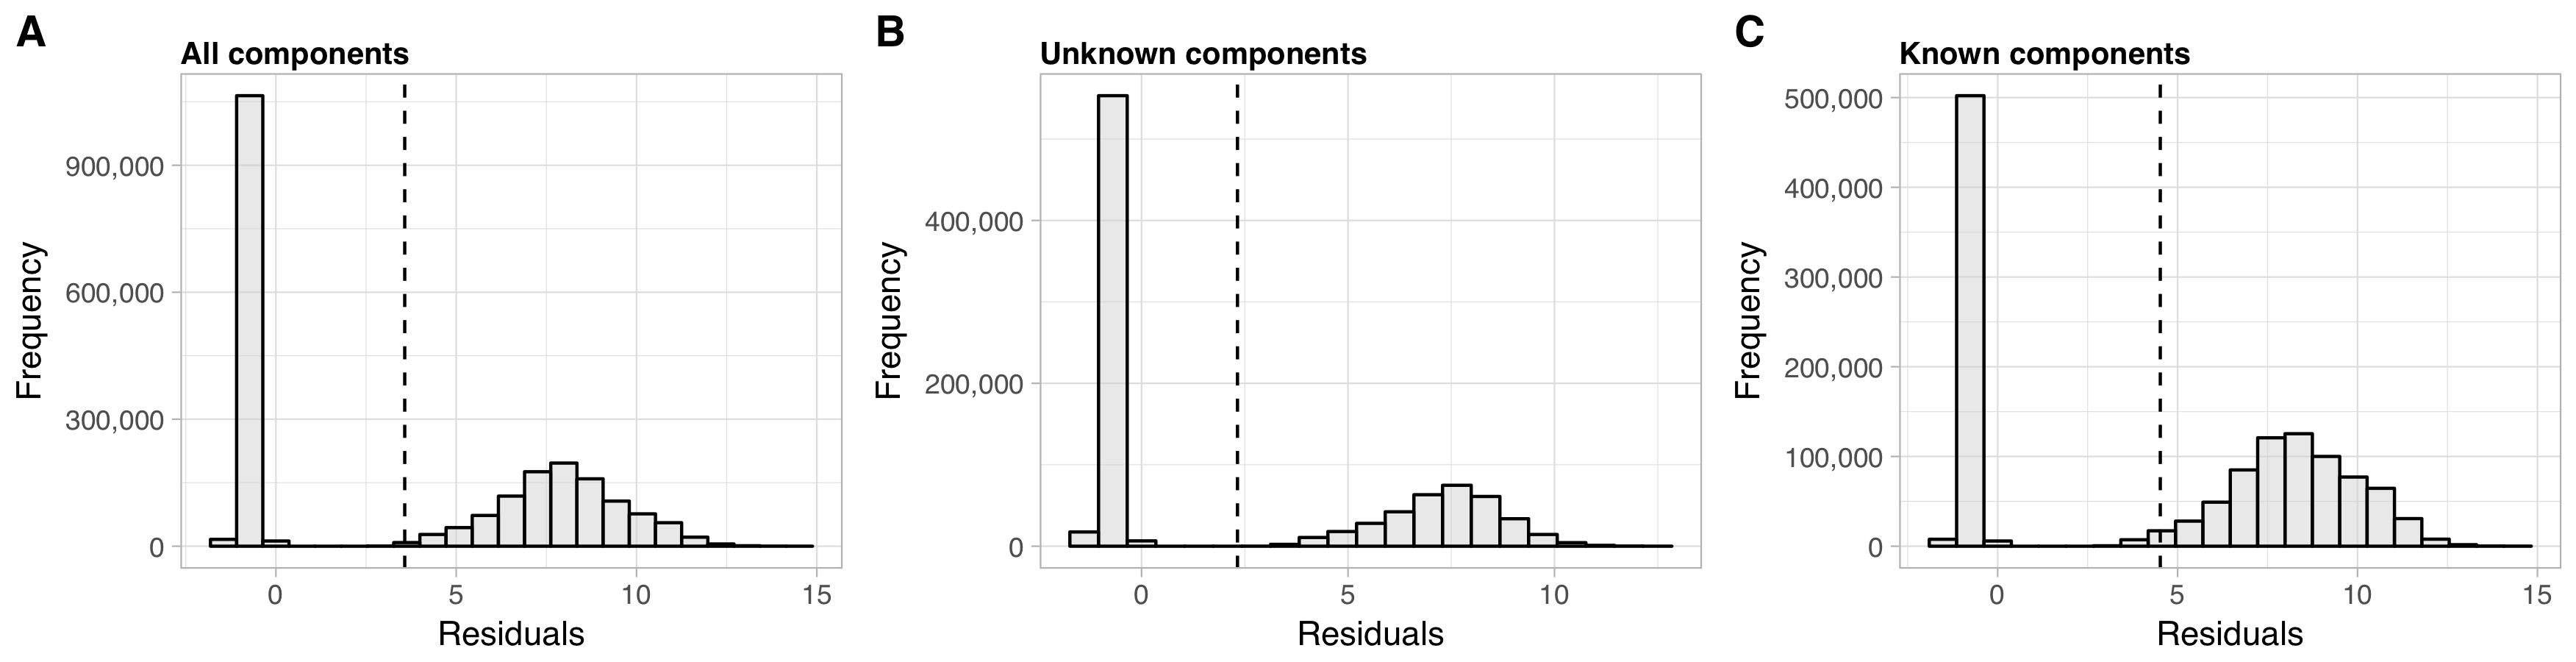
\includegraphics[width=1.0\textwidth] {fig_s1}
	\caption[TARA Oceans PCA residuals histogram]{\textbf{TARA Oceans PCA residuals histogram.} A) Residuals of PCA with sites defined by all components. B) Residuals of PCA with sites defined by at the unknown components (EUs + GUs). C) Residuals of PCA with sites defined by the Known components (K + Kwp).}
	\label{Fig:A1}
\end{figure}

\begin{figure}[h!]
	\centering
	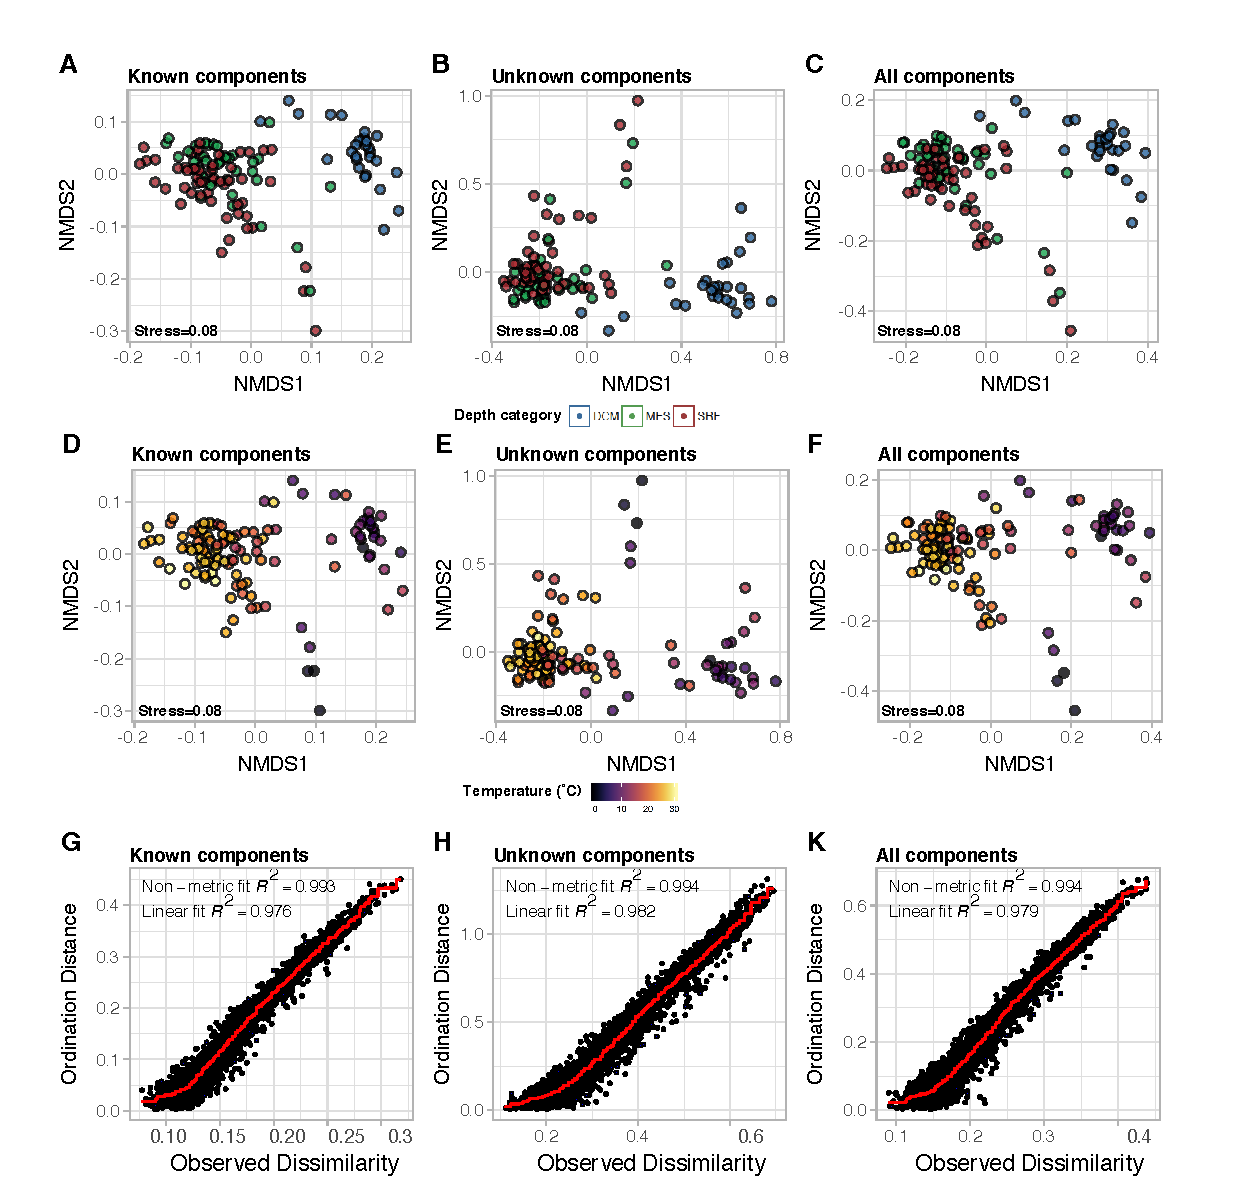
\includegraphics[width=1.0\textwidth] {nmds_panel.pdf}
	\caption[TARA Oceans NMDS and Shepard Plots]{\textbf{TARA Oceans NMDS and Shepard Plots.} A-C) TARA ocean metagenomes defined by (A) Knowns (K + Kwp), (B) Unknowns  (EUs + GUs), and (C) ALL components. Sites are colored by depth of origin (Red = surface, Green = deep chlorophyll maximum, and Blue = mesopelagic. D-E) Same plots as A-C but colored by temperature. The darker the color, the colder the sea water temperature. G-I) Shepard plots for NMDS in A-F }
	\label{Fig:A2}
\end{figure}

\end{appendices}
